\documentclass{beamer}
\usetheme{metropolis} % Use metropolis theme

\usepackage[utf8]{inputenc}
\usepackage[T1]{fontenc}
\usepackage[british]{babel}
\usepackage[autostyle, english = british]{csquotes}
\usepackage[%
  backend=biber,
  doi=false,
  url=false,
  isbn=false,
  eprint=false,
  style=authoryear,
  hyperref=true,
  maxnames=2,
  minnames=1,
  maxbibnames=99,
  firstinits,
  uniquename=init]{biblatex}
\addbibresource{../bibliography.bib}

\usepackage{caption}
\usepackage{xpatch}
\usepackage{bm}
\usepackage{amsmath}
\usepackage{mathtools} % for \mathclap
\usepackage{varioref}
\usepackage{hyperref}
\usepackage[noabbrev]{cleveref}
\newcommand{\creflastconjunction}{, and\nobreakspace} % use Oxford comma
\usepackage{todonotes}
\usepackage{multimedia}
\usepackage{tikz}
\usetikzlibrary{arrows, positioning, shapes.geometric}
\usetikzlibrary{calc}
\graphicspath{{../../figures}}

\newcommand{\cn}{\textbf{TODO: Citation}}

\title{Data-Driven Models for Zebrafish Motion\\IDP kick-off}
\author{Lukas Krenz}
\date{January 12, 2018} 

\begin{document}
\maketitle
\begin{frame}{What \textit{\&} Why?}
Collaboration with Max Plank Institute for Ornithology

Advisers: Jacob (Max Plank), Nicola (CAMP)

Goals:
\begin{enumerate}
\item Compare three models for zebrafish motion
\item Example use case: virtual reality for fish
\end{enumerate}
\end{frame}
\begin{frame}{Zebrafish: Burst-and-coast Motion} 
    \begin{figure}[H]
    \centering
    \movie[width=0.66\textwidth, height=0.66\textwidth, autostart,, loop, poster]{}{motion_experiment.mp4}
    \caption{Example of zebrafish motion}
    \label{fig:calovi-sim}
  \end{figure}
\end{frame}

\begin{frame}{First Model: Force Based (Calovi)}
Following ideas from Calovi \cn. 

\begin{enumerate}
\item Discrete model, model heading change $\delta \phi$ for kicks
\item Decision process only uses current status
\item Force based, stochastic model
\item Symmetry constraints 
\end{enumerate}

Full model:
\begin{align}
  \label{eq:calovi-model}
  \delta \phi &= \delta \phi_r (r_w) + \delta \phi_w (r_w, \theta_w) + \delta \phi_\text{Att} (d, \psi, \Delta \phi) + \delta \phi_\text{Ali}  (d, \psi, \Delta \phi) \\
  &= \text{noise} + \text{wall avoidance} + \text{attraction} + \text{alignment}
\end{align}
\end{frame}

\begin{frame}{Calovi - Only wall}
Consider no social component:
 \begin{equation}
  \label{eq:calovi-wall_model}
  \delta \phi = \delta \phi_r (r_w) + \delta \phi_w (r_w, \theta_w)
\end{equation}
Symmetry for wall influence:
\begin{equation}
  \label{eq:calovi-wall-symmetry}
   \delta \phi_w (r_w, -\theta_w) =  - \delta \phi_w (r_w, \theta_w)
\end{equation}
Split into force term $f(r_w)$ and odd function $O_r(\theta_w)$ 
\begin{equation}
  \label{eq:calovi-wall-split}
  \delta \phi_w (r_w, \theta_w) = f(r_w)O_w(\theta_w)
\end{equation}
\begin{align}
  \label{eq:calovi-wall-force}
  f(r_w) &= \exp\left( -{(r_w/l_w)}^2 \right) \\
  O(\theta_w) &= \left(a_1 \sin(\theta_w) + a_2 \sin(2  \theta_w)  \right)  \left( b_1  \cos(\theta_w) + \cos(2  \theta_w) \right)
\end{align}
\end{frame}

\begin{frame}
  \frametitle{Calovi - Wall Fit}
  \begin{figure}[H]
    \centering
    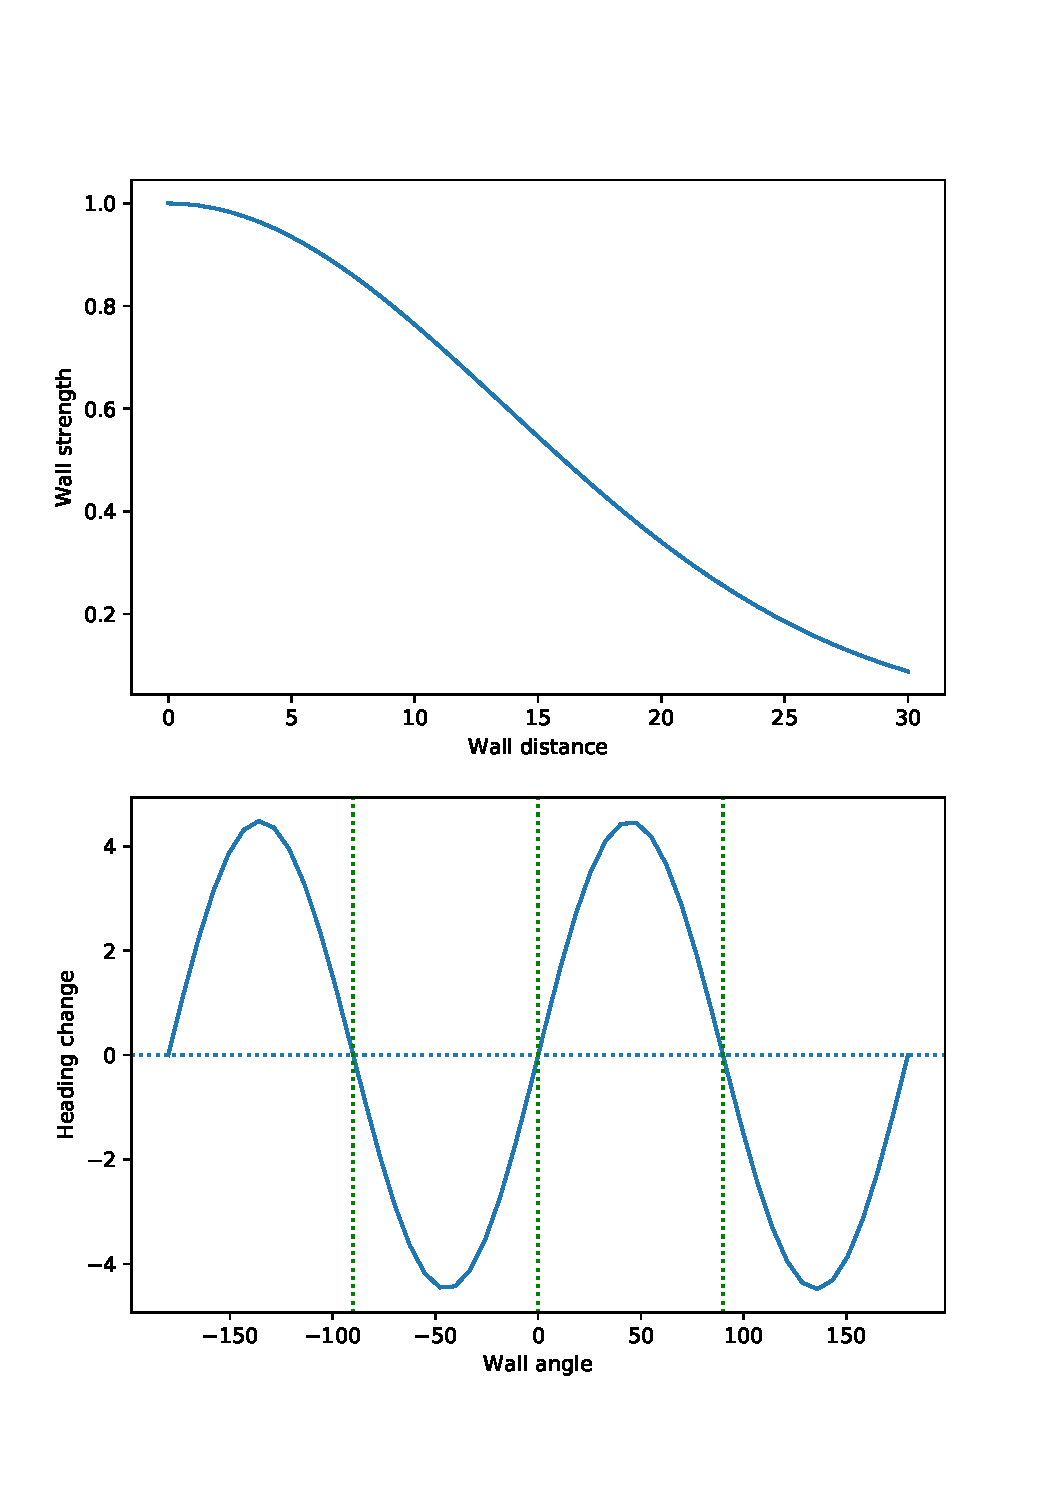
\includegraphics[scale=0.25]{wall_fit.pdf}
    \caption{First results for wall model}
    \label{fig:calovi-sim}
  \end{figure}
\end{frame}

\begin{frame}
  \frametitle{Calovi - First simulation}
    \begin{figure}[H]
    \centering
    \movie[width=0.66\textwidth, height=0.66\textwidth, autostart,, loop, poster]{}{wall_animation.mp4}
    \caption{First results for wall model}
    \label{fig:calovi-sim}
  \end{figure}
\end{frame}

\begin{frame}
  \frametitle{Spatio-Temporal-Receptive Field}
  Inspired by computational neuroscience

  Drop assumption that kick is influenced only by current surroundings
  
  Approximate forces by weighted sum over past environment influences (e.g.\ distances, angles)

  Linear model with memory
\end{frame}

\begin{frame}
  \frametitle{Autoregressive Neural Network}
  Idea: Approximate environment forces with a neural network

  Time series data, strong autocorrelation

  Some evidence for non-linear effects in collective animal motion \cn.

  Use models such as Recurrent Neural Networks (e.g.\ LSTM, GRU) or causal convolutional networks
  
  Highly non-linear model with memory
\end{frame}

\begin{frame}
  \frametitle{Summary}
  \begin{itemize}
  \item Calovi: Linear model without memory
  \item Spatio-Temporal Receptive Field: Linear model with memory
  \item Autoregressive Neural Network: Non-linear model with memory 
  \end{itemize}
\end{frame}
\end{document}